
\documentclass[11pt]{article}
\usepackage{standalone}
\usepackage[margin=0.75in, headheight=20pt]{geometry}

\usepackage{amsmath}
\usepackage{amsfonts}
\usepackage{amssymb}
\usepackage{mathtools}

\usepackage{tikz}
\usepackage{sansmath}
\usetikzlibrary{shadings,intersections}

\usepackage{caption,tabularx,booktabs}

\usepackage{rotating}

\usepackage[utf8]{inputenc}
\usepackage[english]{babel}
\setlength{\parindent}{2em}
\setlength{\parskip}{.25em}
\renewcommand{\baselinestretch}{1.0}

\usepackage{fancyhdr}
\pagestyle{fancy}
\rhead{ Clarke | Blostein | Queen's University}
\renewcommand{\headrulewidth}{0.4pt}
\renewcommand{\footrulewidth}{0.4pt}

\usepackage{courier}

\usepackage[]{algorithm2e}
\usepackage{mathrsfs}

\usepackage{etoolbox}
\patchcmd{\thebibliography}{\chapter*}{\section*}{}{}




\title{Spherical Packing Approach to $\epsilon$-Orthogonal User Selection}
\author{J.E. Clarke, Dr. S.D. Blostein | Queen's University}
\date{Fall, 2018}

\begin{document}
	\maketitle
	\newpage
    \section{Spherical packing approach}
        TODO: Frame the motivation for this approach, cite spherical packing works, outline layout of paper.
        \input{sec1/channel_vectors}
    \section{Projecting vectors to points on spherical surface}\label{sec:chan_norm}
        In order to formulate the problem as a sphere packing problem, channel vectors are assumed to be on the surface of a 2N-dimensional hyper-sphere. That is, the norms of each channel vector are assumed to be the same. This is evident from the definition of a hyper-sphere in $N-1$ dimensions:
\begin{equation}\label{eq:sphere_def}
    \begin{aligned}
        S^{N-1} = \lbrace \underline{h_i} \in \mathbb{R}^N \ : \ \Vert \underline{h_i} \Vert = \rho \rbrace
    \end{aligned}
\end{equation}
where $S^{N-1}$ is a $N-1$ hyper-sphere, $\underline{h}_i$ is a $N+1$-length real vector that is being projected from the origin of the sphere, $\mathcal{O}$, to its surface, and $\rho$ is thre radius of the sphere.

In the case of a wireless channel experiencing deterministic path loss and Rayleigh fading, this assumption is not practically realistic. If path loss is not exactly the same for each vector, the channel norms will differ between vectors (implying they would fall on the surface of different spheres, or some other arbitrary shape). Similarly, the stochastic nature of the channel vectors due to fading will have a similar result.

However, if we assume channel state information at the transmitter (CSIT), the path loss can be estimated and accounted for (neglecting any estimation error in path loss, and assuming power control). Furthermore, the probability that $\Vert \underline{h_i} \Vert^2$ exists in the spherical shell defined by lower and upper radii, $\rho^-$ and $\rho^+$, respectively, is non-zero and can be easily calculated as a function of fading statistics and $\rho^-,\ \rho^+ $. An illustration of the members of this family of spheres is illustrated in Fig. $\ref{fig:concentric_sphere}$.

\begin{figure}
    \centering
    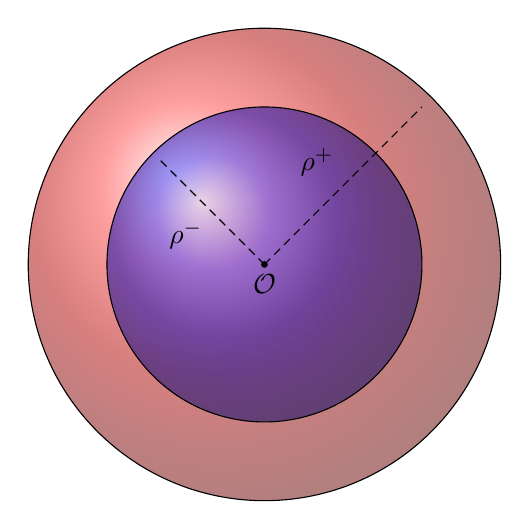
\begin{tikzpicture}
      \coordinate (O) at (0,0);
      
      % outer ball background color
      \shade[ball color = red, opacity = 0.5] (0,0) circle [radius = 3cm];
    
      %outer ball ball
      \draw (O) circle [radius=3cm];
    
      % inner ball background color
      \shade[ball color = blue, opacity = 0.5] (0,0) circle [radius = 2cm];
    
      % inner ball
      \draw (O) circle [radius=2cm];
      % label of ball center point
      \filldraw (O) circle (1pt) node[below] {$\mathcal{O}$};
    
      % radius for inner ball
      \draw[densely dashed] (O) to [edge label = $\rho^-$] (-1.33,1.33);
      % radius for outer ball
      \draw[densely dashed] (O) to [edge label = $\rho^+$] (2,2);
      
    
    \end{tikzpicture}
      \caption{Concentric hyper-spheres of radii $\rho^-,\rho^+$. Channel norms are restricted to this range in order to project vectors onto the surface of a hyper-sphere of constant radius. In order to pessimistically lower bound orthogonality probabilities, the larger radius of $\rho^+$ is chosen. The probability channel norms will fall into this range can be described in terms of channel fading statistics.}
    \label{fig:concentric_sphere}
\end{figure}
  
The CDF of the channel norm will be denoted by $F_{\Vert\underline{hi}\Vert^2}(m,\rho)$, where $\rho$ are realizations of the random variable formed by the channel norm. Each term in the $N$-length vector, $\underline{h}_i$ is represented by two iid normal random variables: one for the real part and one for the imaginary part. When forming the L2 norm of the $N$-length vector, each multiplication forms a sum of length four where each of the arguments of the sum are a product of two random variables. Namely, the sum takes the form real$\cdot$real + real$\cdot$imaginary + imaginary$\cdot$real + imaginary$\cdot$imaginary. Thus, the CDF expression becomes:
\begin{equation}\label{eq:ch_sq_cdf_chan}
    \begin{aligned}
        F_{\Vert\underline{hi}\Vert^2}(\rho;m)& = \Gamma_n(2m,m\rho)\\
        &= Pr[\Vert\underline{h}_i\Vert^2 \leq \rho]
    \end{aligned}
\end{equation}
where $\Gamma_n(\cdot)$ is the incomplete normalized gamma function.

The probability that $\Vert\underline{h}_i\Vert^2$ lands in the shell between radii $\rho^+,\ \rho^-$,  is given by the subtraction of the respective CDF expressions:
\begin{equation}\label{eq:p_s}
    \begin{aligned}
        p_s = \Gamma_n(2N,N\rho^-) - \Gamma_n(2N,N\rho^+)
    \end{aligned}
\end{equation}

The issue of resolving the projection of channel vectors onto the surface of a sphere is still not entirely resolved: we have only described the probability the vectors will exist in a shell defined by upper and lower bounding radii. In order to pessimistically bound orthogonality analysis in the upcoming discussion, it is assumed that all the channel norms that exist in the shell are equal to $\rho^+$. In this way, we have a trade-off between probability of channel norms existence and accuracy of orthogonality analysis: as ${(\rho^+-\rho^-)\rightarrow 0},\ p_s\rightarrow 0$; however, as  $(\rho^+-\rho^-)$ grows, so does the inaccuracy in orthogonality analysis.



    \section{$\epsilon$-orthogonality of points on spherical surface}\label{sec:spherical_caps}
        \subsection{Spherical caps and orthogonality}
            Orthogonality between pairs of vectors can be interpreted geometrically on the spherical surface in terms of spherical caps. A spherical cap is formed on the surface of the hyper-sphere of radius $\rho^+$ by by first extending the channel vector $\underline{h_i}$ onto the spherical surface as described in Section \ref{sec:chan_norm}. Then a cone, with its apex at $\mathcal{O}$, with half angle $\theta$, centered along the axis of $\underline{h_i}$ is intersected with the spherical surface. This intersection defines a spherical cap. $\mathcal{C}_i$. This process is illustrated in Fig. \ref{fig:spherical_cap}. 

considering a spherical surface with two vectors touching the surface of the sphere at arbitrary points on the sphere. A measure of orthogonality between these vectors can easily be calculated by forming the inner product between these vectors. Alternatively we could form a cone for each vector. The apex of each cone is the origin of the sphere, $\mathcal{O}$. The half angle of each cone is given by $\theta$.

\begin{figure}
\centering
    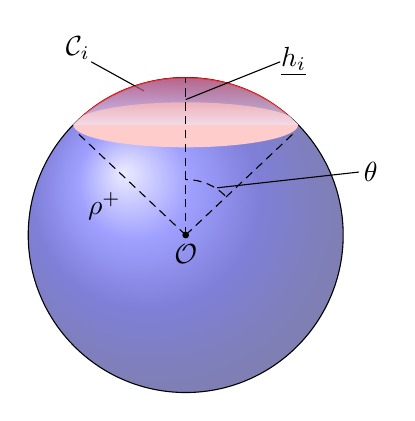
\begin{tikzpicture}%[font = \sansmath]
        %define origin, 1-height of cone, radius
        \coordinate (O) at (0,0);
        \def\r{2}
        \def\H{.6}
        
        \begin{scope}
        % ball background color
        \shade[ball color = blue, opacity = 0.5] (0,0) circle [radius = \r];
        
        % cone
        \begin{scope}
            \def\rx{0.71}% horizontal radius of the ellipse
            \def\ry{0.15}% vertical radius of the ellipse
            \def\z{0.725}% distance from center of ellipse to origin
        
            \path [name path = ellipse]    (0,\z) ellipse ({\rx} and {\ry});
            \path [name path = horizontal] (-\rx,\z-\ry*\ry/\z)
                                        -- (\rx,\z-\ry*\ry/\z);
            \path [name intersections = {of = ellipse and horizontal}];
        
            %% radius to base of cone in ball
            %\draw[fill = gray!50, gray!50] (intersection-1) -- (0,0)
            %  -- (intersection-2) -- cycle;
            %% base of cone in ball
            %\draw[fill = gray!30, densely dashed] (0,\z) ellipse ({\rx} and %{\ry});
        \end{scope}
        
        % label of cone
        %\draw (0.25,0.4) -- (0.9,0.1) node at (1.05,0.0) {$q$};
        
        % ball
        \draw (O) circle [radius=2cm];
        
        % label of ball center point
        \filldraw (O) circle (1pt) node[below] {$\mathcal{O}$};
        
        % radius
        \draw[densely dashed] (O) to [edge label = $\rho^+$] (-1.4,1.32);
        \draw[densely dashed] (O) -- (1.4,1.32);
        %label colatitude angle
        \draw[densely dashed] (0.5,0.5) arc [start angle = 45, end angle = 90, x radius = 7mm, y radius = 7mm];
        \draw (2.2, 0.8) -- (0.4, 0.6) node at (2.35,0.8) {$\theta$};
        
        % cut of ball surface
        \draw[red] (-1.35,1.47) arc [start angle = 140, end angle = 40, x radius = 17.6mm, y radius = 14.75mm];
        %\draw[red, densely dashed] (-1.36,1.46) arc [start angle = 170, end angle = 10,
        x radius = 13.8mm, y radius = 3.6mm];
        %\draw[red] (-1.29,1.52) arc [start angle=-200, end angle = 20,
        x radius = 13.75mm, y radius = 3.15mm];
        
        % label of cut of ball surface
        \draw (-1.2,2.2) -- (-0.53,1.83) node at (-1.37,2.37) {$\mathcal{C}_i$};
        
        %shade the spherical cap
        \begin{scope}
            %clip the shading outside the ball
            \clip ({\r*cos(-90)},{\r*sin(-90)}) arc [start angle=-90,end angle=270,radius=\r];
            %draw the disk    
            \fill[red!20] (0,{\r-\H}) circle [x radius={sqrt(\r^2-(\r-\H)^2)}, y radius={0.2*sqrt(\r^2-(\r-\H)^2)}];
            %shade the disk
            \shade[top color=red!70!gray,bottom color=red!10!blue!10!,opacity=0.6]  ({\r},{1.1*\r}) rectangle ++({-2*\r},{-0.1*\r-\H});
        \end{scope}
    
        %draw channel vector
        \draw[densely dashed] (O) -- (0,2);
        %label channel vector
        \draw (1.2,2.2) -- (0,1.72) node at (1.37,2.2) {$\underline{h_i}$};
        \end{scope}
    \end{tikzpicture}
    
    \caption{Surface of hyper-sphere in 2$N$ dimensions. A spherical cap, $\mathcal{C}_i$ is shown (shaded in red). $\mathcal{C}_i$ is formed by projecting the channel vector, $\underline{h_i}$, onto the spherical surface. A colatitude angle of $\theta$ and radius of $\rho^+$ are assumed in forming $\mathcal{C}_i$. Alternatively, $\mathcal{C}_i$ can also be interpreted as the cap formed by intersecting a cone of half-angle $\theta$ with the spherical surface.}
    \label{fig:spherical_cap}
\end{figure}
        \subsection{Fractional areas and probability of orthogonality}
            Following from the discussion of projecting vectors onto the spherical surface, and defining spherical caps associated with these points, we now extend these concepts the scenario of packing caps onto the surface of the sphere. In this scenario, we assume that vectors are randomly projected onto the surface of the sphere with a uniform density independently from each-other. We would like to know the probability that we can pack $l$ spherical caps of colatitude angle $\theta$ onto the surface of the sphere conditioned on the projection of such vectors onto the surface (as described in Section \ref{sec:chan_norm}). Channel vectors are chosen from a set $\mathsf{A},\ \vert \mathsf{A}\vert = l$ More formally:
\begin{equation}\label{eq:p_perp_cdl}
    \begin{aligned}
        p_\perp &= Pr[\underset{i \in\mathsf{A}}{\cap} \mathcal{P}_j\not\in\mathcal{C}_i\ \forall j\neq i\in\mathsf{A}\ \vert\ \rho^-\leq  \Vert \underline{h_i} \Vert \leq \rho^+,\ \theta ]\\
        &\geq Pr[\underset{i \in\mathsf{A}}{\cap} \mathcal{P}_j\not\in\mathcal{C}_i\ \forall j\neq i\in\mathsf{A}\ \vert\ \Vert \underline{h_i} \Vert = \rho^+,\ \theta ]
    \end{aligned}
\end{equation}
The expression given in Eq. (\ref{eq:p_perp_cdl}) may alternatively be described as the probability that no vector in $\mathsf{A}$ lives in any other vector's spherical cap on the surface $\mathcal{S}^{2N}$, given the vectors live on this surface and a colatitude angle $\theta$. The inequality in $\ref{eq:p_perp_cdl}$ can be explained by the assumed channel norm length of $\rho^+$ for each vector. The channel norms are assumed to be larger than they actually are. Therefore, when the inner product is formed the vectors are assumed to be longer than they actually are. Therefore, their projections onto each-other will be larger than it should be. Thus, the orthogonality constraint is harder to meet.

The probability $p_\perp$ can be expressed in terms of the fractional area of $\mathcal{S}^{2N}$. The probability that any two pair-wise vectors are orthogonal is given by fraction of the area remaining on $\mathcal{S}^{2N}$ after adding $l-1$ cap to the surface. Let $\Omega_{2N}(\rho^+,\theta)$ denote the area of a spherical cap of colatitude angle $\theta$. Therefore the probability that any two vectors are orthogonal on a pair-wise basis is:
\begin{equation}\label{eq:delta_c}
    \begin{aligned}
        \delta_c(\theta,2N) = 2\frac{\Omega_{2N}(\rho^+,\theta)}{\Omega_{2N}(\rho^+,\pi)}
    \end{aligned}
\end{equation}
Thus the area remaining on $\mathcal{S}^{2N}$ after considering one pair of vectors (ie. $\vert \mathsf{A} \vert = 2$) is:
\begin{equation}\label{eq:p_perp_l2}
    \begin{aligned}
        p_{\perp,l=2} = 1-\delta_c(\theta,2N)
    \end{aligned}
\end{equation}

We would like to consider groups of larger sizes (ie. $l> 2$). However, we have the difficulty of determining whether or not the the spherical caps overlap each other. It is important to realize that if the spherical caps $\mathcal{C}_i$ and $\mathcal{C}_j$ intersect each other, it is still possible the vectors are $\epsilon$-orthogonal. However, we know that if $\mathcal{C}_i\cap\mathcal{C}_j = \lbrace \emptyset \rbrace$ the vectors are $\epsilon$-orthogonal since there is no way $\mathcal{P}_j\in\mathcal{C}_i$: the cap $\mathcal{C}_j$ of non-zero radius prevents this case. In this way we can define a lower bound on $p_\perp$, by recalling each vector is projected on the sphere independent from all other vectors, and by assuming each cap is the same size and does not intersect any other cap, the union bound becomes:
\begin{equation}\label{eq:p_perp}
    \begin{aligned}
        p_{\perp} \geq (1-\delta_c(\theta,2N))^{l-1}
    \end{aligned}
\end{equation}
It is important to note that the union bound used in Eq. (\ref{eq:p_perp}) becomes overly pessimistic as the surface of the sphere fills up with caps. The bound does not allow for any caps to intersect at all. However, in reality, it is alright for caps to intersect each other so long as the intersection is not so large that $\mathcal{P}_j\in\mathcal{C}_i$. Allowing some intersection between caps makes packing the sphere much easier as the surface fills up. Therefore for small $N$, large $l$, and/or large $\theta$ the bound in Eq. (\ref{eq:p_perp}) is not expected to be tight.

It has been shown in \cite{Li2011} that the $\delta_c$ function can be realized in terms of an incomplete regularized beta function. Let $\text{I}_z(a,b)$ be the incomplete regularized Beta function. The Beta function is given by the integral:
\begin{equation}\label{eq:beta}
    \begin{aligned}
        \text{B}(a,b) = \int_0^1 t^{b-1}(1-t)^{a-1}dt; \ a>0,\ b>0
    \end{aligned}
\end{equation}

Similarly, the incomplete Beta function is given by:
\begin{equation}\label{eq:beta_inc}
    \begin{aligned}
        \text{B}_z(a,b) = \int_0^z t^{b-1}(1-t)^{a-1}dt; \ a>0,\ b>0,\ z>0
    \end{aligned}
\end{equation}
or alternatively through the integral by making the use of a reparametrization to a polar coordinate system:
\begin{equation}\label{eq:beta_inc_sin}
    \begin{aligned}
        \text{B}_{\sin^2\theta}(\frac{N+1}{2},\frac{1}{2}) = 2\int_0^\theta \sin^N (\phi)\ d\phi; \ a>0,\ b>0,\ \theta>0
    \end{aligned}
\end{equation}

Finally the incomplete regularized function is given by:
\begin{equation}\label{eq:beta_inc_reg}
    \begin{aligned}
        \text{I}_z(a,b) = \frac{\text{B}_z(a,b)}{\text{B}(a,b)}
    \end{aligned}
\end{equation}

We will also make use of the expression for the surface area of an entire hyper-sphere in $N$ dimensions in terms of the Gamma function:
\begin{equation}\label{eq:omega_gamma}
    \begin{aligned}
        \Omega_N(\rho^+,\pi) = \frac{2\pi^{N/2}}{\Gamma(N/2)}(\rho^+)^{N-1}
    \end{aligned}
\end{equation}

As is illustrated by Li in \cite{Li2011}, the area of a spherical cap in $N$ dimensions can be calculated by integrating the surface of a sphere in $N-1$ dimensions along the arc of a great circle with radius $\rho^+\sin\phi$. Where the arc element along the great circle is given by $\rho^+d\phi$. This integral can be expressed in terms of the Beta function given above.
\begin{equation}\label{eq:cap_integral}
    \begin{aligned}
        \Omega_N(\rho^+,\theta) &= \int_0^\theta \Omega_{N-1}(\rho^+\sin\phi,\pi)\ \rho^+d\phi\\
        &= \frac{2\pi^{N-1/2}}{\Gamma(N-1/2)}(\rho^+)^{N-1}  \int_0^\theta \sin^{N-2}(\phi)d\phi\\
        &= \frac{1}{2} \Omega_N(\rho^+,\pi)\  \text{I}_{\sin^2(\theta)}\bigg(\frac{N-1}{2},\frac{1}{2}\bigg)
    \end{aligned}
\end{equation}
Therefore, comparing the expressions in Eqs. (\ref{eq:cap_integral}), (\ref{eq:delta_c}), we arrive at the following expression for $\delta_c$ in terms of the incomplete regularized Beta function:
\begin{equation}\label{eq:delta_c_beta}
    \begin{aligned}
        \delta_c(\theta,2N) = \text{I}_{\sin^2(\theta)}\bigg(\frac{2N-1}{2},\frac{1}{2}\bigg)
    \end{aligned}
\end{equation}

Thus, the bound on $p_\perp$ from Eq. (\ref{eq:p_perp}) can be expressed in terms of $\text{I}_{\sin^2(\theta)}$:
\begin{equation}\label{eq:p_perp_beta}
    \begin{aligned}
        p_{\perp} \geq \bigg(1-\text{I}_{\sin^2(\theta)}\bigg(\frac{2N-1}{2},\frac{1}{2}\bigg)\bigg)^{l-1}
    \end{aligned}
\end{equation}
    \section{$\epsilon$-orthogonal group existence probability}
        \subsection{Sum of dependent random indicator variables}
            In Section \ref{sec:chan_norm} we described a method of approximately projecting channel vectors onto a spherical surface. In Section \ref{sec:spherical_caps} we used this the event of this projection as a condition for developing a probability that a set of $l$ vectors, $\mathsf{A}$, is $\epsilon$-orthogonal. In this section we set out to extend these results further by considering a larger set of candidate vectors, $\mathsf{C} \ :\ \vert \mathsf{C} \vert = m >l$. This result is particularly useful because it allows us to consider the probability that we can find a group of $l$ vectors that are $\epsilon$-orthogonal as a function of the number of candidates we consider, $n$. One would expect that as more candidates are considered for addition to an $\epsilon$-orthogonal group of size $l$, the probability that such a group meets the constraints and attains minimum size $l$ increases with $n$. However, as more candidates are considered, the complexity associated with forming the $\epsilon$-orthogonal group also increases. 

We can describe the collection of $\epsilon$-orthogonal sets using the criteria developed in the previous sections. Let $\mathsf{S}_\epsilon$ be a collection of $\epsilon$-orthogonal sets. $\mathsf{S}_\epsilon$ is formed by testing all subsets of the set of candidate vectors, $\mathsf{A}\subset\mathsf{C}\ : \ \vert \mathsf{A} \vert = l$, against the channel norm and orthogonality constraints previously developed. Thus, $\mathsf{S}_\epsilon$ is a collection of $l$-length sets. The vectors contained within each of these $l$-length sets are mutually $\epsilon$-orthogonal. In the case that $\mathsf{S}_\epsilon = \lbrace \emptyset \rbrace$, no $\epsilon$-orthogonal sets of cardinality $l$ exist in the set of candidate vectors $\mathsf{C}$. This can be expressed more formally as:
 \begin{equation}\label{eq:S_e}
    \begin{aligned}
        \mathsf{S}_\epsilon = \lbrace \mathsf{A}\ \big|\ | \underline{h_j}^H\underline{h_i} |\ <\ \epsilon \ \text{;} \ \rho^-<\Vert \underline{h_i} \Vert^2 < \rho^+\ \forall \ i \neq j \in \mathsf{A} \rbrace \ \forall \mathsf{A}\subset \mathsf{C}
    \end{aligned}
\end{equation}

The purpose of this discussion is to provide an expression for the probability $Pr[\mathsf{S}_\epsilon \neq \lbrace \emptyset \rbrace]$. We adopt the following notation to describe this probability.
 \begin{equation}\label{eq:p_epsilon}
    \begin{aligned}
        p_\epsilon = Pr[\mathsf{S}_\epsilon \neq \lbrace \emptyset \rbrace]
    \end{aligned}
\end{equation}
More specifically, we want to describe $p_\epsilon$ as a function of $l,\ n,\ \theta$. In order to work up to this result, let us first consider the case that $n=l$. In this case, there is only one non-null subset of $\mathsf{C}$, that is, $\mathsf{C}$ itself. Therefore, the existence probability of $\epsilon$-orthogonal set can be stated in terms of Eqs. (\ref{eq:p_s}), (\ref{eq:p_perp_cdl} or \ref{eq:p_perp_beta}) by recalling that $p_s$ is independent of $p_\perp$:
 \begin{equation}\label{eq:p_epsilon_l}
    \begin{aligned}
        p_{\epsilon,l=n} = p_\perp p_s^l
    \end{aligned}
\end{equation}

However, in the case that $n>l$, we must now consider more than one subset of $\mathsf{C}$. In order to do so, we define the the indicator random variable that returns a binary value indicating whether or not $\mathsf{A}\in \mathsf{S}_\epsilon$:
 \begin{equation}\label{eq:orth_indicator}
    \begin{aligned}
        \textbf{1}_{\mathsf{A}} = 
        \begin{cases}
            1,& \text{if } \mathsf{A} \in \mathsf{S}_\epsilon\\
            0,              & \text{otherwise}
        \end{cases}
    \end{aligned}
\end{equation}

The number of $\epsilon$-orthogonal sets in the collection $\mathsf{S}_\epsilon$ may be expressed in terms of a sum of these indicator variables:
 \begin{equation}\label{eq:indicator_sum}
    \begin{aligned}
        K_\epsilon^{(l)} = \sum_{\mathsf{A}\subset\mathsf{C}}1_{\mathsf{A}} \ : \ \vert \mathsf{A} \vert = l
    \end{aligned}
\end{equation}
One can also observe that the expression given in Eq. ($\ref{eq:p_epsilon}$) is equivalent to $Pr[ K_\epsilon^{(l)} \neq 0]$.

It is very important to note at that the argument from one iteration of the sum to the next in Eq. (\ref{eq:indicator_sum}) are not necessarily independent. This follows from the fact that the arbitrary subsets of $\mathsf{C}$ may have intersections. Therefore, the random variables that correspond to these sets will also be dependent. For example, consider tow subsets of $\mathsf{C}$, $\mathsf{A}\subset\mathsf{C}$ and $\mathsf{B}\subset\mathsf{C}$. In the case that $\mathsf{A}\cap\mathsf{B} = \lbrace \emptyset \rbrace$, the the indicator random variables $1_{\mathsf{A}}$ and $1_\mathsf{B}$ will also be independent. However, when $\mathsf{A}\cap\mathsf{B} \neq \lbrace \emptyset \rbrace$, then the random variables $1_{\mathsf{A}}$ and $1_\mathsf{B}$ are mutually dependent. It is important to account for this dependence for the sake of developing an accurate bound on $p_\epsilon$. An approach based on random graphing and dependence graphing, similar to \cite{Swannack2005}, \cite{Janson2004} will be taken to overcome this problem.
        \subsection{Random graphs and dependence graphs}
            The graph approach taken will be as follows. Firstly, a graph will be generated based on the multiplication of the channel matrix and its conjugate transpose (Hermitian). The resulting square matrix is then transformed based on the channel norm and orthogonality constraints given in Eq. (\ref{eq:S_e}). Such an approach is the same taken by \cite{SwannackThesis}. The transformed elements that remain in the matrix after this are then interpreted as a graph which can be used to quantify the sum given in Eq. (\ref{eq:indicator_sum}) using the method given by \cite{Janson2004}.

Let us define $H$ as the channel matrix whose columns are the channel vectors corresponding to the set of candidate vectors $\mathsf{C}$. Therefore, $H$ is a $N \times m$ matrix. Next let us define the $m \times m$ square matrix given by the product of $H$ with its conjugate transpose:
 \begin{equation}\label{eq:w_matrix}
    \begin{aligned}
        W = H^HH
    \end{aligned}
\end{equation}
At this time, take a moment to note what the elements of $W$ represent. The diagonal elements of $W$ are the L2 norms of the channel. The off-diagonal elements are the inner products between the various channel vectors. Therefore, the elements of $W$ may be compared to the constraints given in Eq. (\ref{eq:S_e}). More specifically, the diagonal elements may be compared to the channel norm requirements in terms of $\rho^-,\ \rho^+$, and the off-diagonal elements may be compared to the orthogonality constraints in terms of $\epsilon$ or $\theta$.

Motivated by these constraints, we define the transforms $\mathfrak{T}_\rho$ and $\mathfrak{T}_\theta$ that operate on square matrices such as $W$. Let $w_{ii}$ be the $i^{the}$ diagonal element of $W$, and let $w_{ij}$ be the element of $W$ at the $i^{th}$ row, $j^{th}$ column.

The transform, $\mathfrak{T}_\rho(W;\ \rho^-, \ \rho^+)$, transforms $W$ into a new $\Hat{m}\times \Hat{m}\ : \ \Hat{m}\leq m$ square matrix, $\Hat{W}$, by appending rows and columns of $W$ depending on the corresponding diagonal element $w_{ii}$ that belong to the $i^{th}$ row and column. If $\rho^- \leq w_{ii}\leq \rho^+$ holds, then the $i^{th}$ row and column of $W$ are appended to the transformed matrix $\Hat{W}$. However, if this condition does not hold, then the $i^{th}$ row and column are not appended to $\Hat{W}$: instead they are appended to the set $\mathsf{P}_\rho$. That is, $\mathsf{P}_\rho$ is the set of all vectors that do not meet channel norm requirements. Once all the diagonal elements in $W$ have been considered, all the diagonal elements in $\Hat{W}$ are set to 1.

The transform $\mathfrak{T}(\Hat{W};\ \theta)$, operates on the off-diagonal elements of $\Hat{W}$. The result of the transform is a $\Hat{m}\times\Hat{m}$ square matrix, $\Tilde{W}$, whose elements take binary values 0 or 1. While $\mathfrak{T}_\rho$ removed rows and colums associated with diagonal elements, $\mathfrak{T}_\theta$ quantizes off-diagonal elements of $\Hat{W}$ to binary values of 0 or 1. If $\vert \Hat{w}_{ij} \vert <\cos\theta$, then $\Hat{w}_{ij}$ is set to 1; otherwise, it is set to 0. Note that $\Tilde{W}$ is a symmetric matrix by virtue of the hermitian operation and transforms used to generate the matrix.

We now interpret the binary elements as a description of the graph $\Gamma(\Tilde{W},\mathsf{P}_\rho$ . We begin by interpreting the elements along the diagonal of $\Tilde{W}$ as vertices of $\Gamma$. Next, we form an edge between the $i^{th}$ vertex associated with $\Tilde{w_{ii}}$ and the $j^{th}$ vertex associated with $\Tilde{w_{ij}}$ if the value of $\Tilde{w}_{ij}=1$. Edges are formed throughout the graph by repeating this process for all the diagonal elements of $\Tilde{W}$, making comparisons to all the elements that belong to $\Tilde{w}_{ii}$'s row. Finally a vertex is added to the graph corresponding to each element in the set $\mathsf{P}_\rho$. There are no edges to the vertices associated with $\mathsf{P}_\rho$.

Let us take a moment to draw connections between the graph $\Gamma$ and the expression given in Eq. ($\ref{eq:S_e}$). The number of vertices in the graph is the same as the cardinality of the set of candidate vectors $\vert \mathsf{C}\vert = m$. The collection of sets $\mathscr{S}_\epsilon$ in Eq. (\ref{eq:S_e}) can be represented in $\Gamma$ by forming $\mathscr{A}$ which is the collection of $\binom{m}{l}$ sets (or $l$-tuples), $\mathsf{A}$, on the vertices of $\Gamma$, regardless of whether or not edges exist, then testing against channel norm and orthogonality constraints in terms of indicator variables. The graph interpretation can be related to $1_{\mathsf{A}}$ in terms connectivity between vertices. If the $l$-tuple of vertices, $\mathsf{A}\subset\Gamma$ is fully connected (ie. edges exist between vertices in the tuple such that one can travel to any vertex), then   $1_{\mathsf{A}} = 1$, otherwise $1_{\mathsf{A}} = 0$.

We can now relate this to the work done by Janson \cite{Janson2004} to quantify the expression in Eq. (\ref{eq:indicator_sum}) using the graph $\Gamma$. It is important to note before proceeding that $1_\mathsf{A}$ is a Bernoulli-distributed random variable, which takes value 1 with probability $p_\perp$. Further, a requirement of using the following expressions from $\cite{Janson2004}$ is that $1_\mathsf{A}$ and $1_\mathsf{B}$ are independent so long as there is no intersections between the sets $\mathsf{A}$ and $\mathsf{B}$. This may seem like a redundant statement; however, if the random variables upon which $1_\mathsf{A}$ and $1_\mathsf{B}$ are correlated, this statement does not hold. However, in our case, we assume independent Rayleigh fading. The random variables contained within each vector are iid, and the vectors themselves are independent. Therefore, we meet this requirement.

Two upper bounds are given on probabilities relevant to our application in \cite{Janson2004}. Firstly Theorem 2.1 gives:

 \begin{equation}\label{eq:pr_janson_thrm_2-1}
    \begin{aligned}
        Pr[K_\epsilon^{(l)} \leq \text{E}\lbrace K_\epsilon^{(l)} \rbrace -t] \leq \exp\bigg(\frac{-2t^2}{\chi^*(\mathscr{A})\vert \mathscr{A}\vert}\bigg)
    \end{aligned}
\end{equation}
Secondly, Corollary 2.4 gives:
\begin{equation}\label{eq:pr_janson_corollary_2-4}
    \begin{aligned}
        Pr[K_\epsilon^{(l)} \leq \text{E}\lbrace K_\epsilon^{(l)} \rbrace -t] \leq \exp\bigg(\frac{-8t^2}{25\chi^*(\mathscr{A})p\vert \mathscr{A}\vert}\bigg)
    \end{aligned}
\end{equation}
where $p$ is the probability associated with $1_\mathsf{A}$ taking a value of 1. $\chi^*$ is the fractional chromatic number of the graph formed by the set of vertices and edges $\mathsf{A}\in\Gamma$.

In our case, we are particularly interested in the case $Pr[K_\epsilon^{(l)} = 0]$ as in Eq. (\ref{eq:p_epsilon_sum}). In order to arrive at this result we will manipulate the expressions given in Eqs. (\ref{eq:pr_janson_thrm_2-1}),(\ref{eq:pr_janson_corollary_2-4}). 

Firstly, we notice that the sum of Bernoulli random variables will result in a binomial distribution for $K_\epsilon^{(l)}$. The mean of the binomial distribution, regardless of dependence in the sum, is given by:
\begin{equation}\label{eq:binom_mean}
    \begin{aligned}
        \text{E}\lbrace K_\epsilon^{(l)} \rbrace &= \vert \mathscr{A} \vert p
        =\binom{m}{l}p
    \end{aligned}
\end{equation}
We also note that $p=p_\perp$. Additionally, it can be shown as in \cite{Janson2004} Example 4, so long as the conditions of independence hold as described above, $\chi^*(\mathscr{A})$ can be bounded:
\begin{equation}\label{eq:chi_bound}
    \begin{aligned}
        \chi^*(\mathscr{A})\leq\chi^*(\Gamma)\leq \frac{ \binom{m}{l}}{\lfloor \frac{m}{l} \rfloor}
    \end{aligned}
\end{equation}

Thus, following from Eq. (\ref{eq:pr_janson_thrm_2-1}):
\begin{equation}\label{eq:pr_thrm_2-1}
    \begin{aligned}
        Pr[K_\epsilon^{(l)} \leq 0] &\leq \exp\bigg(\frac{-2p_\perp^2\binom{m}{l}^2}{\frac{\binom{m}{l}}{\lfloor \frac{m}{l}\rfloor}\binom{m}{l}}\bigg)\\
        &= \exp\bigg( -2p_\perp^2 \lfloor \frac{m}{l} \rfloor \bigg)\\
        &\geq Pr[K_\epsilon^{(l)} = 0]
    \end{aligned}
\end{equation}

Similarly, following from Eq. (\ref{eq:pr_janson_corollary_2-4}):
\begin{equation}\label{eq:pr_corollary_2-4}
    \begin{aligned}
        Pr[K_\epsilon^{(l)} \leq 0] &\leq \exp\bigg(\frac{-8p_\perp^2\binom{m}{l}^2}{25\frac{\binom{m}{l}}{\lfloor \frac{m}{l} \rfloor} p_\perp \binom{m}{l}} \bigg)\\
        &= \exp\bigg(\frac{-8p_\perp \lfloor \frac{m}{l} \rfloor}{25} \bigg)\\
        &\geq Pr[K_\epsilon^{(l)} = 0]
    \end{aligned}
\end{equation}

Finally to guarantee an upper bound on $ Pr[K_\epsilon^{(l)} = 0]$, we have:
\begin{equation}\label{eq:pr_K_ub}
    \begin{aligned}
        Pr[K_\epsilon^{(l)} = 0]&\leq \exp\bigg(-\text{max}\bigg\lbrace \frac{8p_\perp \lfloor \frac{m}{l} \rfloor}{25}, 2p_\perp^2 \lfloor \frac{m}{l} \rfloor\bigg\rbrace \bigg)
    \end{aligned}
\end{equation}

Therefore, following from Eqs. (\ref{eq:K_rho}),(\ref{eq:p_epsilon_sum}),(\ref{eq:pr_K_ub}), we have:

\begin{equation}\label{eq:p_e_sum_exp}
    \begin{aligned}
        p_{\epsilon,l,n} = \sum_{j=l}^n \binom{j}{l}p_s^l(1-p_s)^{(j-l)} (1-\exp\bigg(-\text{max}\bigg\lbrace \frac{8p_\perp \lfloor \frac{j}{l} \rfloor}{25}, 2p_\perp^2 \lfloor \frac{j}{l} \rfloor\bigg\rbrace \bigg))
    \end{aligned}
\end{equation}

            %Let us first define the dependecncy graph $\Gamma$. $\Gamma$ is a graph whose vertices are 
    \section{Concluding remarks}
        In this paper we have investigated and expanded upon the spherical packing approach for selecting semi-orthogonal groups of users in a wireless communications context developed in \cite{Swannack2005}. The expression given in Eq. (\ref{eq:p_e_sum_exp}) makes use of several bounds that are not expected to be tight for large group size and strict orthogonality constraints.

The work reviewed here will be used in future work focused on more robust STA-AP association in IEEE 802.11 downlink.
    \newpage

	%\section{Appendices}
	    %\subsection{Notes on Gamma-distributed variables}
	    %    \input{app/gamma_dist.tex}
    \newpage	
 	\begingroup
 		\renewcommand{\section}[2]{}%
 		\bibliographystyle{IEEEtran}
 		\bibliography{references}
 	\endgroup
\end{document}
